\section{IR of Industrial Compilers}
\frame{
\frametitle{IR of Industrial Compilers :: LLVM Bitcode \\
How to generate IR for (field) vars?
}
\begin{columns}
\begin{column}{0.60\textwidth}
\begin{center}
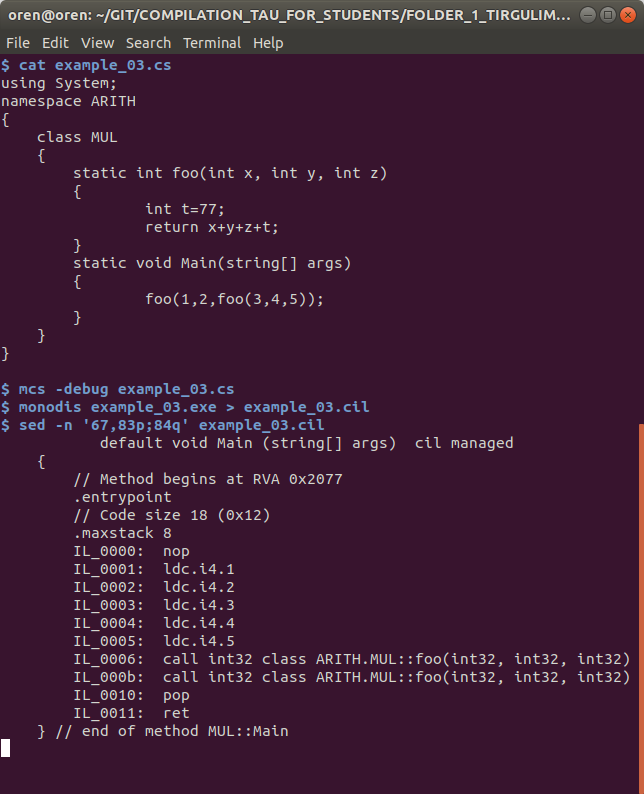
\includegraphics[width=0.95\textwidth]{example_03.png}
\end{center}
\end{column}
\begin{column}{0.6\textwidth}
\begin{itemize}
\item
look at the last command in the {\color{blue} blue}
rectangle: tmp2 := $[$ age $]$
\item
was in synthesized from p$\rightarrow$age?
or from its father \textit{return} node?
\item
To achieve a uniform handling of (field) vars,
they need to \textit{always return their address}.
\item
father nodes (except one, which?)
will add an extra indirection
to extract the content.
\end{itemize}
\end{column}
\end{columns}
}